
\section{Methodology}

\subsection{Intrinsic-Correlation Estimator} \label{methodo:est}

\begin{figure}[t!]
 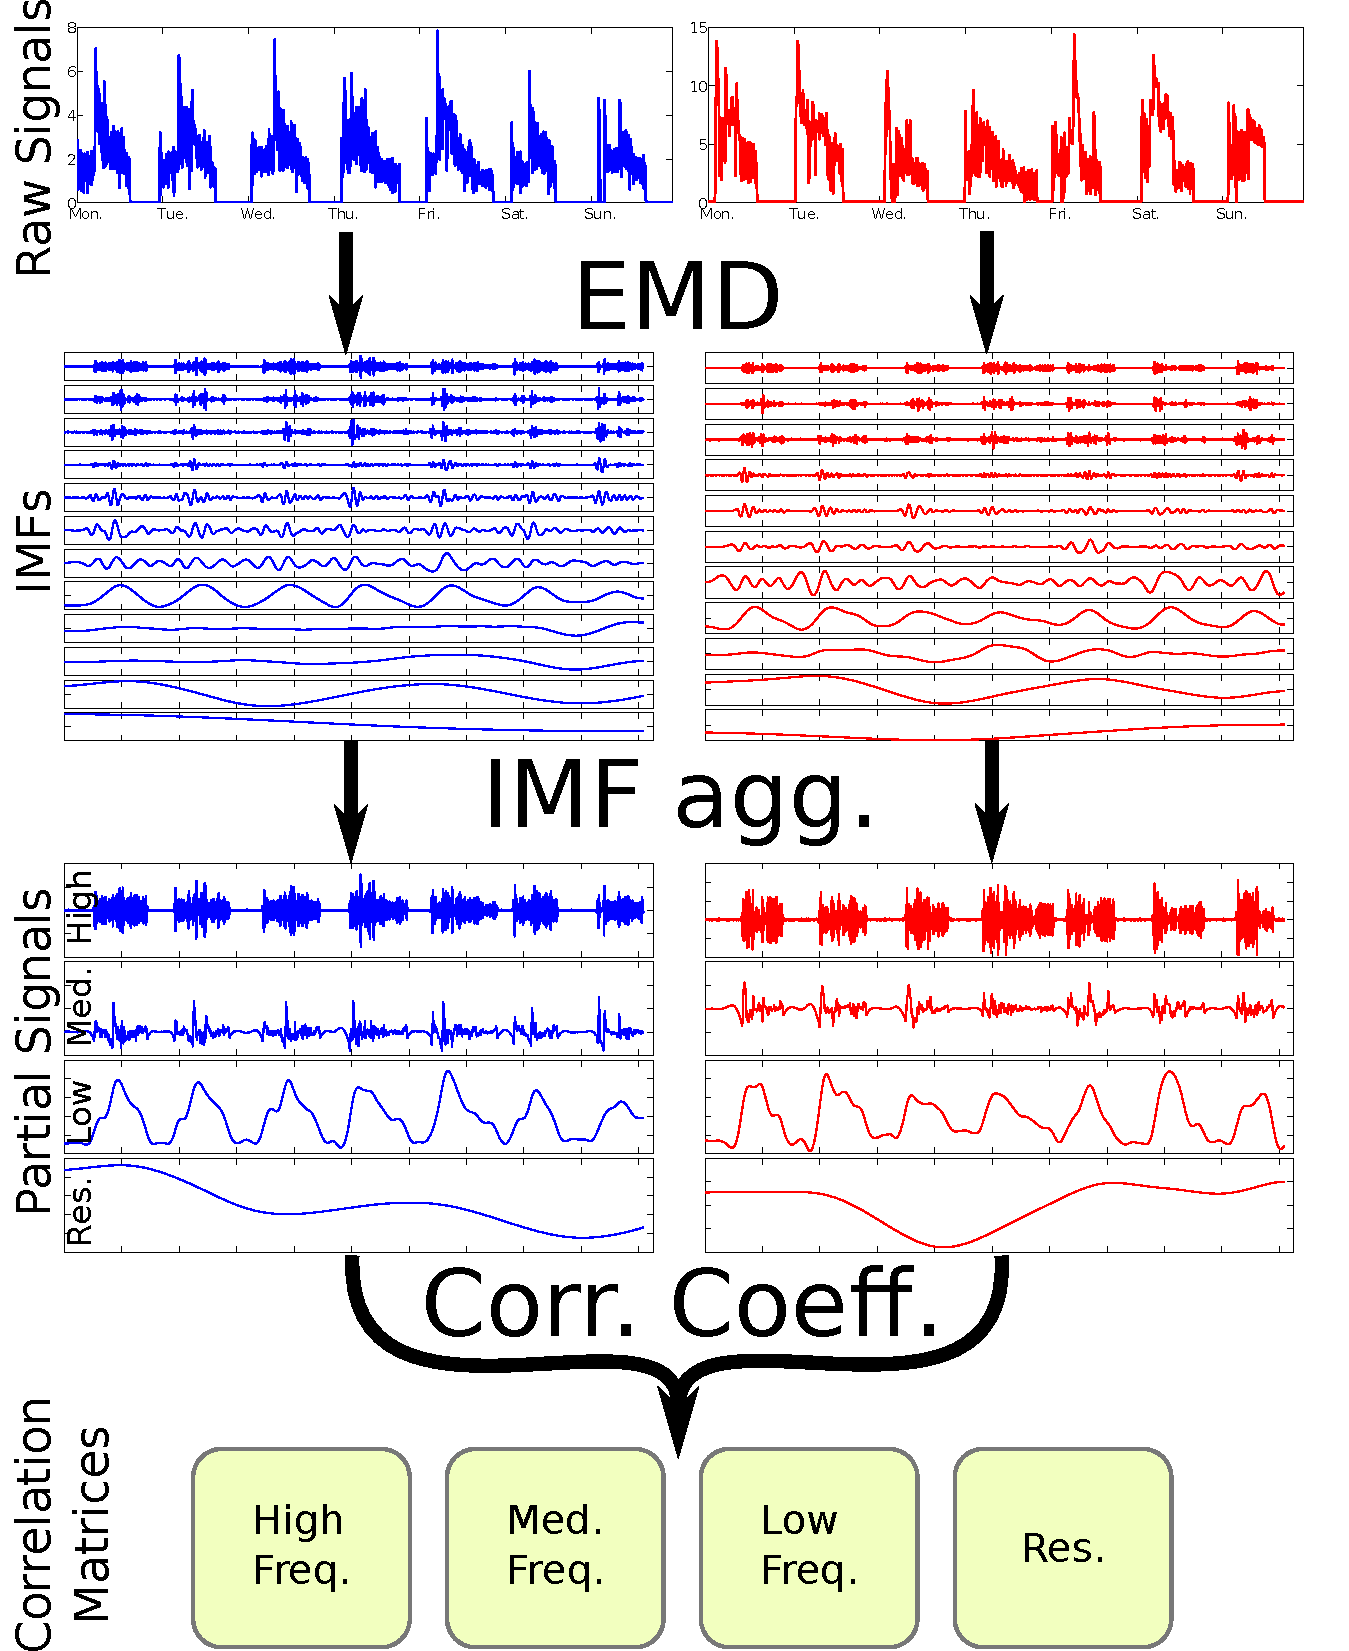
\includegraphics[width=.5\textwidth]{img/estimator.pdf}
 \caption{Overview of the intrinsic-correlation estimator analyzing two raw signals standing for one week of data from two different HVACs. (1)~Decomposition of the two signals in IMFs using EMD; (2)~aggregation of each signal IMFs based on their time scale; (3)~comparison of the partial signals (aggregated IMFs) using correlation coefficient.}
 \label{fig:diagram1}
\end{figure}

As demonstrated in the previous section discovering the devices that are used in concert is particularly difficult due to the dominant pattern of office hours.
The proposed correlation estimator address this issue by decomposing each signal into a set of components, called IMFs, that reveal the data structures at different time scales.
This IMF decomposition is based on a recent signal processing technique: Empirical Mode Decomposition (see \emph{EMD} in Fig.\ref{fig:diagram1}).
The next step is to filter out the IMFs that interfere with our goal and analyze only those standing for time scales shorter than the unwanted daily pattern.
Consequently, the proposed estimator aggregates the IMFs that falls into the same meaningful time scales ranges (see \emph{IMF agg.} in Fig.\ref{fig:diagram1}).
The resulting partial signals from different devices are compared pairwise to identify the devices intrinsic relationships (see \emph{Corr. Coeff.} in Fig.\ref{fig:diagram1}). 

% These intrinsic relations are uncovered by comparing the sensors data at certain meaningful frequency bands.
% Namely, looking at high frequency allows to compare short-term variations representing the instantaneous devices change of state, however, the low frequency highlights long-term fluctuations revealing long devices usage pattern.
% 
% ..... the similarity estimators analyzes the readings from several sensors and reports scores standing for the similarity of the sensors at different frequency bands.
% First, the similarity estimator takes advantage of EMD to decompose the sensors signals into a set of components called intrinsic mode functions (IMFs).
% Second, it constructs band-limited signals by aggregating the IMFs whose mean frequencies fall in a certain frequency band.
% Thereby the pairwise comparison of band-limited signals provides the sensors correlations at different frequency bands. 
% 
% The advantages of the proposed intrinsic-correlation estimator are adaptive approach, ... 

% These two steps are described by the two following sections.

\subsubsection{Empirical Mode Decomposition}
Empirical Mode Decomposition (EMD) \cite{huang:emd1998} is a technique that decomposes a signal and reveals its intrinsic patterns, trend and noise.
This technique has been widely applied to a variety of datasets, including climate variables \cite{barnhart:climateEMD2011,lee:climateEMD2011}, medical data \cite{lima:bioMed2006,echeverria:bioMed2001,blanco:bioMed2008}, speech signals \cite{huang:signalProc2006,hasan:ieeeletter2009}, and images \cite{nunes:image2003,nunes:vision2005}.
% for example, it helped to uncover the global surface temperature trends\cite{}, solar activity patterns and predicts climate variables .
The EMD success relies on its empirical, adaptive and intuitive approach.
In fact this technique is designed to efficiently decompose both non-stationary and non-linear signals without requiring any predetermined basis functions.  

EMD decomposes a signal into a set of oscillatory components called intrinsic mode functions (IMFs). 
An IMF satisfies two conditions: (1) it contains the same number of extrema and zero crossings (or differ at most by one); (2) the two IMF envelopes defined by its local maxima and local minima are symmetric with respect to zero. 
Thereby, the IMFs are functions that directly conveys the amplitude and frequency modulations.

EMD is an iterative sifting process that extracts IMFs step by step; each step seeks for the IMF with the highest frequency, then the computed IMF is removed from the data and the residual data are used as input for the next step.
The process stops when the residual data becomes a monotonic function from which no more IMF can be extracted.

We formally describe the EMD process as follows: 
\begin{enumerate}
\item for a signal \emph{X(t)}, let $m_1$ be the mean of its upper and lower envelopes as determined from a cubic-spline interpolation of local maxima and minima.
\item The first component $h_1$ is computed: $h_1=X(t)-m_1$
\item In the second sifting process, $h_1$ is treated as the data, and $m_{11}$ is the mean of $h_1$'s upper and lower envelopes: $h_{11}=h_1-m_{11}$
\item The procedure is repeated $k$ times, until $h_{1k}$ is an IMF: $h_{1(k-1)}-m_{1k}=h_{1k}$
\item Then it is designated as $c_1=h_{1k}$, the first IMF from the data, which contains the shortest period component of the signal. We separate it from the rest of the data: $X(t)-c_1 = r_1$, and the procedure is
repeated on $r_j: r_1-c_2 = r_2,\dots,r_{n-1} - c_n = r_n$
\item The process stops when $r_n$ contains no more than 3 extrema.
\end{enumerate}

Thereby, the result of EMD is a set of IMFs $c_i$ and the final residue $r_n$, such as: \[X(t)=\sum^{n}_{i=1}c_i+r_n\]
where the size of the resulting set of IMFs $n$ depends on the original signal $X(t)$ and $r_n$ represents the trend of the data (see \emph{IMFs} in Fig.\ref{fig:diagram1}).

For this work we implemented a variant of EMD called Complete Ensemble EMD \cite{torres:icassp2012}.
This algorithm computes EMD several times with additional noise, it allows us to efficiently analyze signals that have flat sections (i.e. consuming no electricity in our case) and permits to solve the EMD mode mixing problem.

\subsubsection{IMF aggregation} \label{methodo:corr}
By applying EMD to power consumption signals we obtain a set of IMFs that precisely describe the devices consumption patterns at different time scales.
Thereby we can concentrate our data analysis on the smaller time scales thus ignoring the daily pattern that prevent us from efficiently analyzing raw signals.

However, comparing the IMFs obtained from different signals is not straightforward.
Because EMD is empirically uncovering IMFs from the data there is no guarantee that the two IMFs $c_i^1$ and $c_i^2$ obtained from two distinct signals $S^1$ and $S^2$ represent data at the same time scale.
Directly comparing $c_i^1$ and $c_i^2$ is meaningless unless we confirm that they belongs to the same time domain.

There is numerous techniques available to retrieve the IMFs frequencies \cite{huang:aada2009}.
In this work we take advantage of the Generalized Zero Crossing (GZC) \cite{huang:patent2006} because it is a simple and robust estimator of the IMF instantaneous frequency \cite{huang:aada2009}.
GZC is a direct estimation of the IMF instantaneous frequency using critical points defined as the zero crossings and local extrema (round dots in Figure \ref{fig:gzc}).
Namely, given a data point $p$ GZC measures the quarter ($T_4$), the two halves ($T_2^x$) and the four full periods ($T_1^y$) $p$  belongs to (see Figure \ref{fig:gzc}) and the the instantaneous period is computed as:
\[T=\frac{1}{7}\{4T_4+(2T_2^1+2T_2^2)+(T_1^1+T_1^2+T_1^3+T_1^4)\}\]

\begin{figure}
\begin{center}
 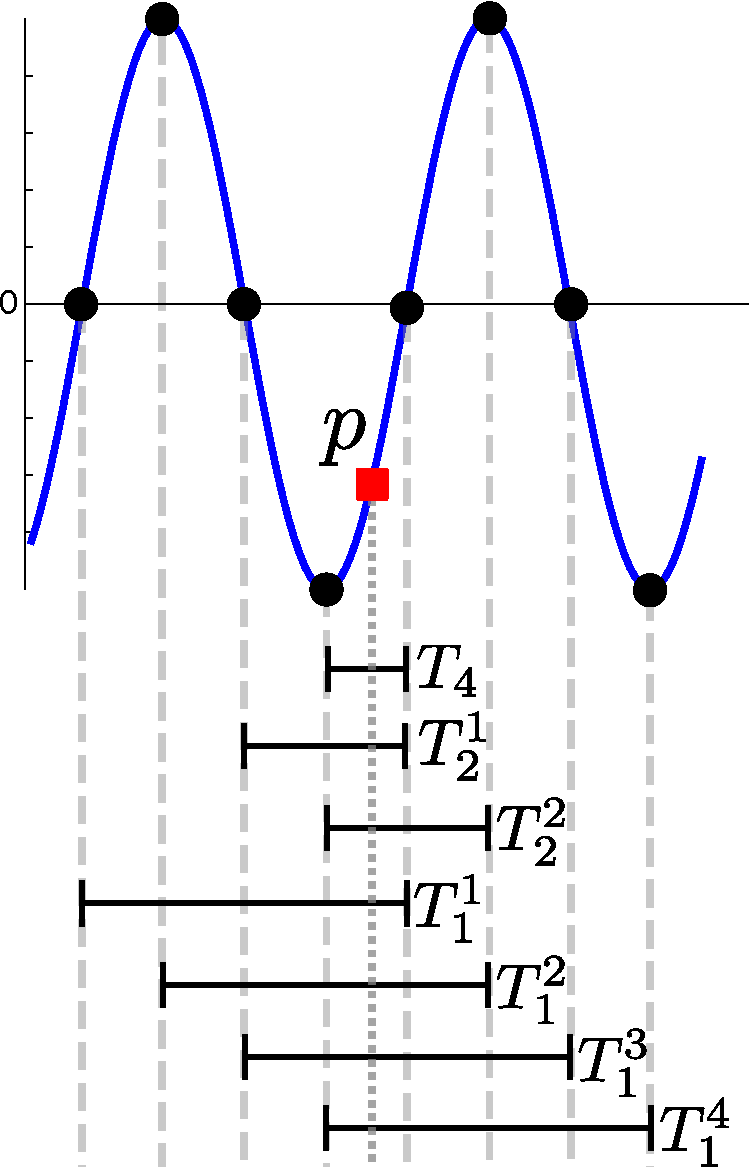
\includegraphics[width=.3\textwidth]{img/gzc.pdf}
 \end{center}
 \caption{Generalized Zero Crossing: the local mean period at the point $p$ is computed from one quarter period $T_4$, two half periods $T_2^x$ and four full periods $T_1^y$ (where $x=1, 2$, and, $y=1,2,3,4$).}
 \label{fig:gzc}
\end{figure}

Thereby GZC provides the instantaneous period for each couple of consecutive critical points.
Hereafter we refer to the time scale of an IMF as the average of the instantaneous periods along the whole IMF.

EMD inherently extracts IMFs at different time scales that depend on the original signal.
In order to efficiently compare IMFs obtained from different signals we partially reconstruct the signals by aggregating IMFs that fall into the same time scale range.
Thereby, two partial signals standing for the same time scale range can be directly compared.

We define four time scale ranges: 
\begin{itemize}
 \item the \emph{high frequencies} stand for all the IMFs with a time scale lower than 20 minutes. These IMFs capture the noise and observational errors.
 \item The \emph{medium frequencies} stand for all the IMFs with a time scale between 20 and 360 minutes. These IMFs convey the devices usage.
 \item The \emph{low frequencies} stand for all the IMFs with a time scale between 360 and 8640 minutes. These IMFs represent the daily usage of the devices.
 \item The \emph{residual data} is all data with a time scale higher than 8640 minutes. This is mainly the residual data obtained after applying EMD and it highlights the trend of the devices.
\end{itemize}

These time scale ranges are arbitrarily determined according to our experiments and goal.
Namely, the 20 minutes boundary relies on the sampling period of our dataset (5 minutes) and permits to capture IMFs with really short periods.
The 360 minutes (i.e. 6 hours) boundary allows us to analyze all patterns that have a period shorter than the usual office hours.
The 8640 minutes (i.e. 6 days) boundary allows us to capture daily patterns and week days pattern.

Thereby, for each device we obtain 4 partial signals representing different characteristics of the device power consumption (see \emph{Partial Signals} in Fig.\ref{fig:diagram1}).
We compare the devices pairwise using the correlation coefficient of their partial signals.
In the example of Figure \ref{fig:diagram1}, the correlation coefficient of the raw signals suggests that they are highly correlated ($0.5675$). 
However, the comparison of the corresponding partial signals provides new insights;
the two devices are poorly correlated at high and medium frequencies (respectively $-0.0127$ and $-0.0420$) but highly correlated at low frequencies (0.7886) meaning that these devices are not intrinsically correlated but only features similar daily pattern.

All the devices are compared pair wise at the four different time scale ranges.
Consequently we obtain four correlation matrices that monitor the devices similarities at different time scales.
Each line of these matrices (or column as the matrices are symmetric) reveals the behavior of a device, namely, its relationships with the other devices at a certain time range scale.
These matrices are our system fundamental tools to track the behavior of the devices and permit the proposed anomaly detector to identify misbehavior.


\subsection{Anomaly Detector}\label{methodo:ano}
The proposed anomaly detector aims at identifying devices misuses in an unsupervised manner.
The devices activity is monitored via the correlation matrices presented in the previous section.
Using numerous observations the detector computes an adaptive reference that exhibits the normal devices utilization.
Then the detector compares the computed reference with the current data and reports devices that deviate from their usual behavior.

\subsubsection{References computation}
We define four reference matrices that exhibit the normal devices behavior at the four time scale ranges defined in the Section \ref{methodo:corr}.
These references are similarly computed; (1) we retrieve the correlation matrices for $n$ consecutive time bins of length $l$ as described in the Section \ref{methodo:est}. (2) For each pair of devices we store the median correlation over the $n$ time bins and obtain a matrix of the median device correlations.

Formally, for each time scale range the computed reference matrix for the $d$ devices and the $n$ time bins is:
\[\tilde{R}_{i,j} =  \median(C^1_{i,j},...,C^n_{i,j})\]
where $i$ and $j$ ranges in $[1,d]$.

Assuming that the devices predominantly behave normally and the anomalies are exceptional events, the reference matrices exhibit the normal device behaviors.
In fact the abnormal correlation values that could appear in the $n$ analyzed time bins are ignored by the median operator thanks to his robustness to the outlier values.

\subsubsection{Behavior change}
The anomaly detection consists in identifying the devices that have a behavior significantly different from the one provided by the reference matrices.
Consequently, we compare each device behavior for a certain time bin to the one provided by the reference matrix.

Consider the correlation matrix $C^t$ obtained using the data from the time bin $t$.
Then, the vector $C^t_{i,*}$ is the behavior of the $i^{th}$ device for this time bin.
In addition, its normal behavior is given by the corresponding vector in the reference matrix; $R_{i,*}$.
We exhibit the device behavior change at the time bin $t$ with the following Minkowski weighted distance;

\[ l^t_{i} = \left(\sum_{j=1}^p  w_j\left(C^t_{i,j} - R_{i,j}\right)^k\right)^{1/p} \]

where $w_j$ is defined as;

\[ w_j = \frac{R_{i,j}}{\sum_{k=1}^d R_{i,k}} \]

The weight $w_j$ permits to prioritize the relationship changes with the intrinsically-correlated devices given by the reference matrix.
In other words, our definition of behavior change is mainly driven by the relationship alterations among devices that are usually highly correlated.
We also set $p=4$ in order to inhibit small differences between $C^t_{i,j}$ and $R_{i,j}$ and emphasize the main distinction with the reference matrix.

By monitoring this quantity over numerous time bins the abnormal device behaviors are easily identified as the outlier values.
In order to identify these outlier values we implement a robust detector based on MAD, a robust dispersion measure commonly used in anomaly detection \cite{huber:wiley2009,chan:springer2005}.

MAD stands for \emph{median absolute deviation} and it is a measure that robustly estimates the variability of the data by computing the median of the absolute deviations from the median of the data.
Namely, let $l_{i}$ be a vector representing the behavior changes of the device $i$ over numerous time bins, then its MAD value is defined as:
\[ \mad_i = b \median(\lvert l_{i} - \median(l_{i})\rvert)\]
where the constant $b$ is usually set to $1.4826$ for consistency with the usual parameter $\sigma$ at Gaussian distributions.

Thereby we define as anomalous the behavior change of the device $i$ at the time bin $t$ that satisfies the following equation;
\[l^t_{i} > \median(l_{i}) + \tau  \mad_i\]
where $\tau$ is a parameter that permits to make the detector more or less conservative.

The final output of the proposed detector is a list of alarms in the form $(t,i)$ meaning that the device $i$ has an abnormal behavior at the time bin $t$.
The priority of the alarms in this list is selected by the building administrator by tuning the $\tau$ parameter.
